\chapter{Introduction}
\label{chapter1}

Climate change calls for a shift to renewable energy and restructuring of the electric power industry.
Source \cite{eurostat2020} shows that as of the time of reading this paper, 44 \% of produced electricity in Europe was from combustible sources such as gas, fuel, and coal. Even 
though that is a significant decrease of 10 \% in the last 10 years, it is a significant Co2 emitter.
The same source \cite{eurostat2020} also states that a third of energy is consumed by the residential sector. It is estimated, 
that the human population will reach 10 billion inhabitants in the next 10 years, and ever-increasing ownership of electrical appliances such as smartphones, HVACs, and EVs will further elevate this issue.
Acknowledging this, reducing consumption in the residential sector could leave a significant impact on the human footprint. 

%increased time spent indoors*

The EU aims to be climate neutral by 2050, therefore it seeks to improve the efficiency of every part of pollution contributors through The European Green Deal.
A large part of these contributors is the Energy sector.
A subpart of the energy sector is the residential sector, where many advancements could be made to help to reach the goal.  

This could be achieved through various applications and methods that use load profiling as their core technology.
Authors in paper \cite{Chuan2014} proposed a method to reduce peak loads by studying consumer
appliance usage patterns. Paper \cite{Csoknyai2019} studied consumer usage patterns, and returned feedback that contributed to reducing consumption.
Another notable way is the use of distributed energy resources and managing them in such a way as to decrease the net output of energy flow such as the authors describe in
\cite{MORENOJARAMILLO2021445}. All described methods would reduce and alleviate the load off the power grid.

Load profiling in building energy consumption is not a novelty and had been in research since the 1980s.
While it was thought that aggregated LPs of households are relatively predictable, recent data obtained using smart meter data showed large deviance from user to user due to different lifestyles, as the author states in paper \cite{Review2021}.
In recent years LPs have changed due to renewable energy accelerated development of distributed energy resources such as residential photovoltaic
power plants, home wind energy, and using EVs with home batteries. Socioeconomic changes such as work-from-home, also drastically reshaped the LP curve. 

The thesis aims to propose and develop new, previously unused LPs, that will contribute to mitigating the raised issues. 
Before we disclose our contributions, let us first have an overview of what LPs are and in which other use cases they can be utilized, besides the energy saving that we just mentioned.

% finishing words here 

\section{Definition and Types of LPs}
\label{sec:LP_types}
Author \cite{Review2021} defines terms as following:

% definiton
% usage
% analysis

\begin{itemize}
	\item Load: the electricity that all the electricity-powered devices in the household consume in unit time.
	\item Profile: a graph representing the significant features of the electricity load over time.
\end{itemize}

In other words, LPs are a graphical presentation of the consumption features of a building over time. 
Here, features could be anything that presents consumption. 
In most cases that is power.
The time range used to present the consumption could be anything from daily, weekly, monthly to yearly.

One thing to mention here is, that although the buildings were mostly consuming energy in the past, nowadays, they also producing it.
While this may beak the definition of LPs, it makes them even more useful, since they can be used to present electricity production as well.
Even though, throughout the thesis, we will relate it mostly to electricity consumption.
\subsection{Feature Set} 
\label{ssec:feature_set}

If we want to find the base features, we have to look at how consumption measurements are done in most buildings. 
The following three features enable us to know the amount of energy being consumed by the user.

\begin{figure}[H]
  \Tree[.base\ features [.power ]
          [.timestamp ]
          [.name ]
                ]
\end{figure}

If we translate these features to the time domain and observe them over a specified amount of time, new ones emerge. 
The most notable example is the observation of electrical power over one hour.
The result is energy $E$, and it is one of the most common ways used to bill a customer for his power consumption.

We can also extract features such as the number of activations or time of operation for each activation.
This can be done using sensors to detect activity or even extract this from power consumption data.
In cases where we are observing individual appliances, this can be done using simple signal processing
techniques. In cases where we are observing buildings, this could be achieved using more complex disaggregation algorithms also known as NILM algorithms.
This additional processing and equipment is a downside that we have to keep in mind when we are comparing it to power data.
% Time domain
\begin{figure}[H]
  \Tree[.time\ domain\ features [.energy $E$ ]
          [.number\ of\ activations $N_{act}$  ]
          [.operating\ time $t_{oper}$  ]
                ]
\end{figure}

\begin{figure}[H]
	\centering
	\caption{Simple signal processing of power consumption for a single appliance}
	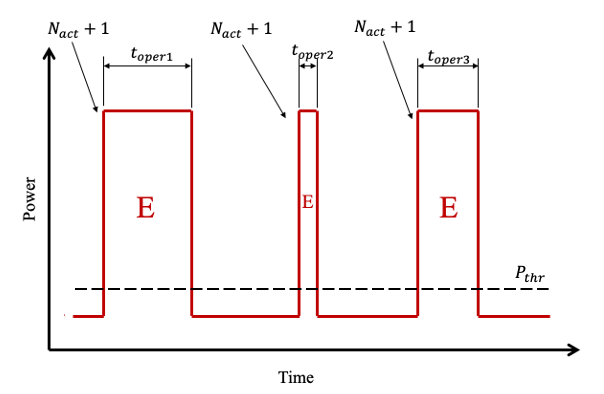
\includegraphics[width=0.9\textwidth]{Figures/profile_sketches/singal_processing_thr.png}
	\label{fig:sig_proc_fig}
\end{figure}

As we can see in Figure \ref{fig:sig_proc_fig} all three-time domain features can be extracted from the graphical presentation. 
Energy $E$ is equal to the area under the graphical presentation or in other words integral of power over time. 
$N_{act}$ can be measured based on the number of times the power value exceeded some pre-defined threshold $P_{thr}$. 
The $t_{oper}$ is the time between on and off events, where we use the same threshold as with $N_{act}$.
While there are other features, such as time between activations, or total operational time that could be
extracted, these were not commonly used in related work.

% \begin{figure}[H]
% \Tree[.frequency\ domain\ features [.Operation\ Modes ]]
% \end{figure}
% The same as we can present power in the time domain, the same can be done in the frequency domain. 
% One actual example can be seen in Figure \ref{fig:freq}.
% Here, it is hard to extract more features, but one possibility could be
% detecting the number of operation modes based on the number of peaks, using signal processing algorithms.

% \begin{figure}[H]
% 	\centering
% 	\caption{Frequency of power values for the toaster. Actual data from the REFIT dataset.}
% 	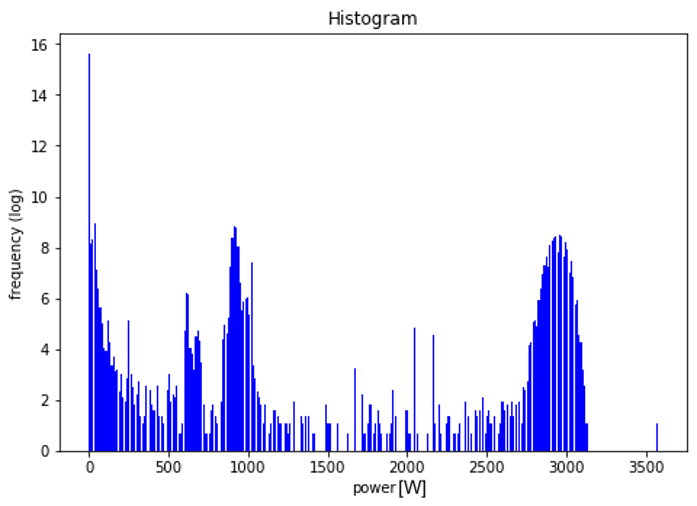
\includegraphics[width=0.9\textwidth]{Figures/profile_sketches/freq.png}
% 	\label{fig:freq}
% \end{figure}

% In the case of Figure \ref{fig:freq} we are observing a toaster over one year.
% Toasters are usually simple appliances using a heating element and a thermostat, meaning that the power consumption should be constant and set by the resistance of the heating element.
% The Figure shows \ref{fig:freq} a nice normal distribution of power values around 3 kW, 
% which we can assume is the heating element.
% We can notice two other peaks one at roughly 1 kW and the other at 0.7 kW.
% Since toasters usually do not have operation modes, we could assume that there 
% are other appliances plugged into the metering device, 
% meaning this could be a use-case for this kind of LP.

\subsection{Types of LPs} 

\subsubsection{Power LP}
\label{ssec:feature_set}

Combinations of the features result in many possible types of LPs that enable us to present the data.
The most commonly used type of LP is average power consumption over some time.
One such example can be seen in Figure \ref{fig:daily_power_profile}. 
Here, we used daily timescale, since it is so commonly used it is also known as the standard daily LP. 
This LP can be used to portray per-building as well as per-appliance data.
Its use is one of the most versatile, and it is used in fields such as demand response, anomaly detection and zero-energy buildings.
While the LP in Figure \ref{fig:daily_power_profile} is a sketch, it still presents consumption trends in morning and evening peaks.
% ad usage and then analysis
\begin{figure}[H]
	\centering
	\caption{Average daily usage profile for an appliance or a building}
	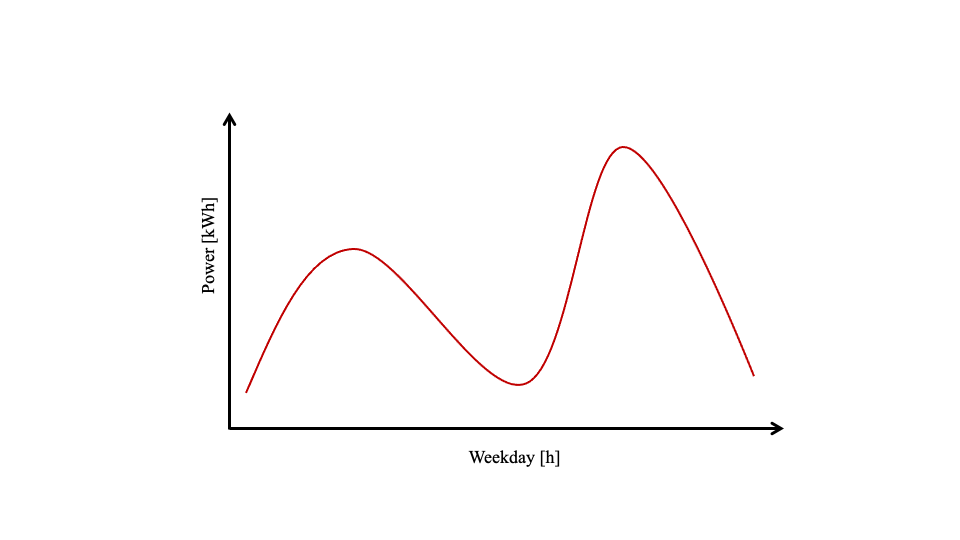
\includegraphics[width=0.9\textwidth]{Figures/profile_sketches/Slide1.png}
	\label{fig:daily_power_profile}
\end{figure}

\subsubsection{Activation LP}
Alternatively, we can use a histogram-based presentation to present a number of activations feature such as can be seen in Figure \ref{fig:daily_act_profile}.
Here, we split the given timescale into discrete intervals also known as buckets. 
These buckets are then filled with activations that had taken place in a given interval. 
In the case of Figure \ref{fig:daily_act_profile} timescale is a day and it was split into 12 intervals.
While this is not real-world data we can again observe consumption patterns throughout the day, with morning and evening peaks. 
activation LP is usually used to portray per-appliance data. 
In order to portray per-building data, we would need to install a power meter for every appliance in the building.
This LP has the very same use-cases as the power type and can be used in the same fields, but as mentioned, it is less practical for per-building LPs.
While Figure \ref{fig:daily_act_profile} presents the same data as Figure \ref{fig:daily_power_profile},
due to data processing, it could potentially reveal more relevant consumption patterns.
The downside is that we have to invest additional time to process power data into activations.

\begin{figure}[H]
	\centering
	\caption{Histogram of daily activations profile for an appliance or a building}
	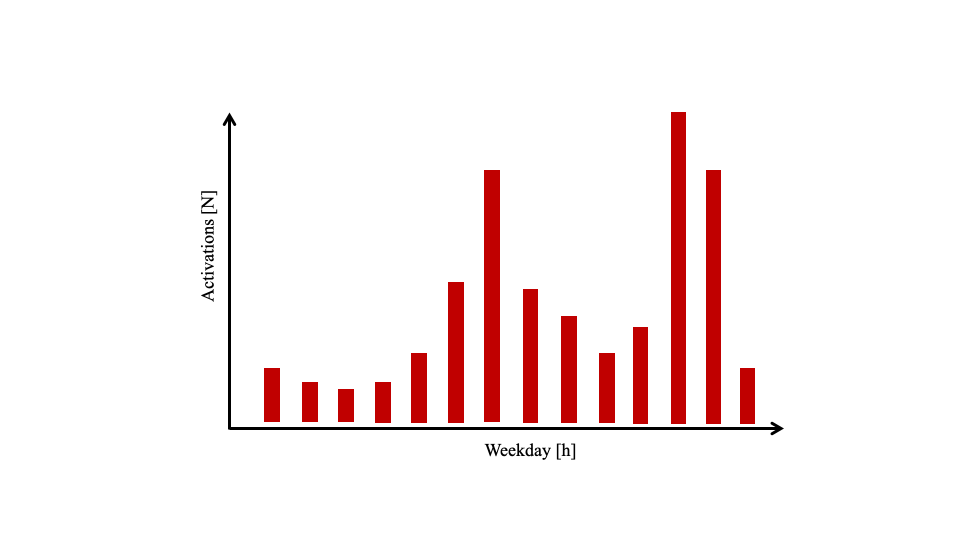
\includegraphics[width=0.9\textwidth]{Figures/profile_sketches/Slide5.png}
	\label{fig:daily_act_profile}
\end{figure}

\subsubsection{Per-Building Per-Appliance LP}
The next two types of LP are known as per-building per-appliance LPs.
They can be used to present whole building usage as well as per-appliance consumption. 
Two such examples can be seen in Figure \ref{fig:daily_act_m_profile} and \ref{fig:daily_power_m_profile}.
In the case of activation LP, we concatenate activations of each appliance and label them accordingly.
This enables us to see the contribution of each appliance to the total number of activations in each bucket.
The per-building per-appliance LPs have the potential to be used in the same fields as the first two types, but practically they are only used in demand response.
Additional information enables us to understand the data and potentially discover patterns that we otherwise would not be able to.
The reason behind slow adoption could be that this additional information is not needed.

\begin{figure}[H]
	\begin{subfigure}{.5\textwidth}
		% \centering
		\caption{Daily per-building per-appliance activations LP for appliances A and B}
		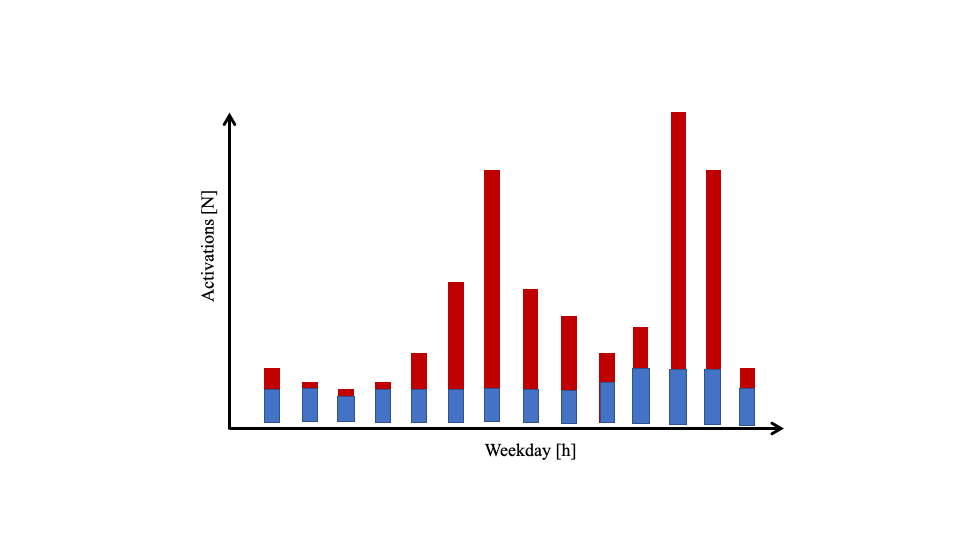
\includegraphics[width=1.1\textwidth]{Figures/profile_sketches/Slide8.png}
		\label{fig:daily_act_m_profile}
	\end{subfigure}%
	~ 
	\begin{subfigure}{.5\textwidth}
		% \centering
		\caption{Daily per-building per-appliance power LP for appliances A, B and C}
		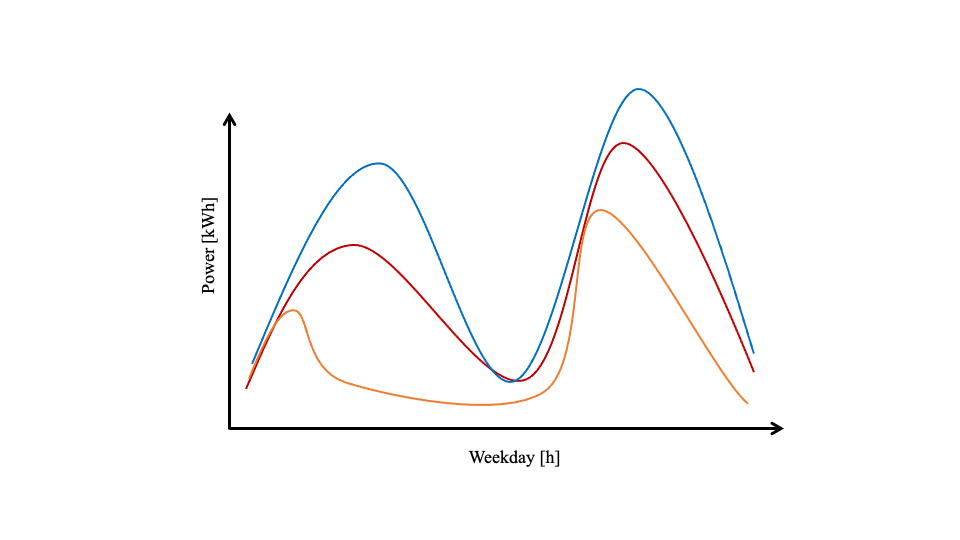
\includegraphics[width=1.1\textwidth]{Figures/profile_sketches/Slide2.png}
		\label{fig:daily_power_m_profile}
	\end{subfigure}%
	\label{fig:daily_m_profile}
	\caption{Per-building Per-appliance LP}
\end{figure}

\subsubsection{Heatmap LPs}

The last type is a heatmap LP. 
Heatmap LPs can be further divided into two subtypes.

The first type is LPs which consist of two-time dimensions and use color to display consumption.
This LP can be used to portray activation as well as power consumption features and could be used to present per-building consumption as well as per-appliance data.
All this makes them very versatile.
One such example can be seen in Figure \ref{fig:heatmap_2dtime}. 
It is possible to see the consumption pattern throughout each day in a month.
The brightness presents the activity of the household or an appliance. 
The brighter the plot, the more activity for that hour of that day of the month.
One other thing to keep in mind when reading such a profile is that the origin is placed in the upper left corner.
This originates from image processing standards.

\begin{figure}[H]
	\centering
	\caption{Number of daily activations/power consumption of one appliance/house in one-month period}
	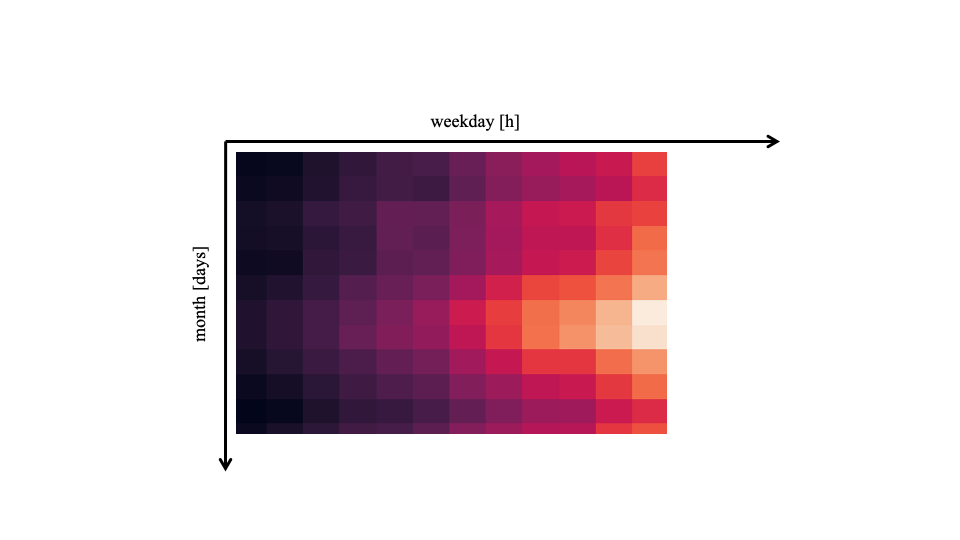
\includegraphics[width=0.9\textwidth]{Figures/profile_sketches/Slide10.png}
	\label{fig:heatmap_2dtime}
\end{figure}

The second subtype is essentially Per-building Per-appliance LP but portrayed differently.
Instead of plotting consumption data as the sum of contributions of each appliance, we plot their consumption by side.
These LPs have the same uses as Per-building Per-appliance LPs since they are essentially the same.
One such sketched example can be seen in Figure \ref{fig:heatmap_all_appl}.

\begin{figure}[H]
	\centering
	\caption{Consumption for each appliance in a day}
	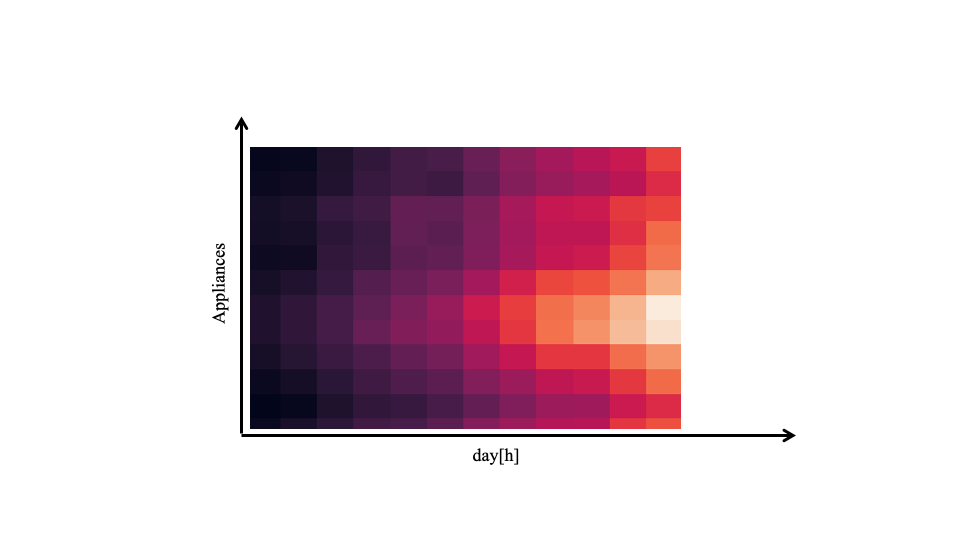
\includegraphics[width=0.9\textwidth]{Figures/profile_sketches/Slide12.png}
	\label{fig:heatmap_all_appl}
\end{figure}

While there are many features and many more types of LPs out there, we have selected the ones that are most commonly used.
There are also many versions of the LPs above with different timescales, where each has a different use case.
A more detailed presentation of use cases will also follow in the coming chapters, with a classification in the next section.

\section{LP Use-cases}
\label{sec:use_cases_tree}

\begin{figure}[H]
	% \caption{General classification of LP use-cases}
	\label{tree:clasification_of_use_cases}
	\Tree[.{LP Use\ Cases} 
	[.Grid\\Managment Energy\\saving Zero\\Energy\\Buildings Demand\\response ]
	[.Anomaly\\Detection Elderly\\Care Fault\\Detection ]
	[.Other Develo-\\pment\\Feedback Occupancy\\Detection Energy\\Stealing ]
		]
\end{figure}

The load profiling method has a lot of different use cases across different fields.
In our case, we will split use cases into three classes.

The first class is grid management.
For example, it can be used to save energy by studying users' usage patterns and returning feedback, with suggestions on how to improve consumption.
In cases where buildings have grid batteries and PV installed, the same feedback could be used to minimize the amount of energy being pulled from the grid.
These are so-called zero-energy buildings (ZEB).
Electrical energy providers could use demand response programs in combination with the LPs to optimize the management of the grid, with minimal impact on users' daily lives.

The second class is anomaly detection.
The LPs could be used to help the elderly in case of an accident or even help prevent one. 
They could be used to detect all kinds of early malfunctions in the operation of appliances, which would reduce service costs and save energy.

The last class is other, where occupancy detection, development feedback and energy stealing are all cases where LPs could be used. 

A more detailed description of each use-case with publications will be addressed in the next chapter in section \ref{sec:use-cases}

\section{Data}
\label{sec:data}
To construct the LPs we used 5 different datasets.
These are UK-DALE \cite{UKDALE}, REFIT \cite{REFIT}, ECO \cite{ECO}, REDD \cite{REDD}, and iAWE \cite{iAWE}.
All datasets measured electrical energy consumption in residential buildings.
They include main smart meter data, as well as sub-meter data for each appliance in a dwelling. 
While some datasets offered versions with high frequency with sampling rates up to 40 kHz,
we focused on the low-frequency variations with sampling rates at around 1 Hz.

The datasets used, had frequencies ranging from 1 Hz for the ECO dataset, down to 1/8 Hz for the REFIT dataset.
For datasets to be compatible, we resampled all datasets to 1/6 Hz.
The missing samples were forward filled with a limit of 5, meaning if up 30 s of data was missing, its value was set to the last known value, otherwise, it was left missing.
For easier handling datasets will be sliced into 1-hour intervals.
The exact methodology will be presented in the methodology Chapter \ref{chapter3}. 

\section{Contributions}
\label{sec:contributions} 

The main goal of the master's thesis is to propose suitable LPs for supporting residential building consumption optimization and elderly care management.
To achieve this goal, we propose the following steps, where each step is a contribution to the scientific community.

\begin{enumerate}
	\item[1.] Surveying the state-of-the-art LPs (Chapter \ref{chapter2})
\end{enumerate}

The first contribution is provided by taking a look at existing research and use-cases. 
Using the publications, we constructed a table of LPs.
We are the first to analyze LPs from this aspect. 
The analysis provides an overview of related work by mapping it to the table.
The table reveals LPs that were not yet utilized.
Using use cases we try to determine in what field each LP could be used.

\begin{enumerate}
	\item[2.] Development of multidimensional activation LPs (Chapter \ref{chapter4})
\end{enumerate}
Empty gaps in research motivated us to pursue the next contribution, 
the development of multidimensional activation LPs. 
Here we offer an in-depth look into the LPs, by presenting the profiles and showing how they present the consumption patterns.
Each LP presents a different pattern and therefore has a different use case. 

\begin{enumerate}
	\item[3.] Visual analysis of activation LP's (Chapter \ref{chapter5})
\end{enumerate}
The third contribution refers to exploratory data analysis (EDA) through visualizations.
Here we leverage proposed and analyzed LPs and t-SNE dimensionality reduction algorithm to understand how data is related.

\begin{enumerate}
	\item[4.] Propose a new anomaly detection method for elderly care (Chapter \ref{chapter6})
\end{enumerate}

This newly obtained knowledge should help us provide the last contribution.
In this chapter, we utilize LPs that haven't been considered before.
We design and construct elderly care assisted living system by utilizing one of the proposed LPs.
The system can detect anomalies in the daily routine of an elder.
In case the anomaly is detected, the caregiver is notified to check on the caretaker. 
It is simple, efficient and ready for real-world use.
